\subsection{Scalability and performance of data centers}

\subsubsection{Evaluate system quality}

System quality information is critical from a cost and performance perspective. In this context, \dquotes{\emph{performance}} means the \textbf{overall effectiveness of a computer system in terms of throughput}, \textbf{response time}, and \textbf{availability}.

\begin{flushleft}
	\textcolor{Green3}{\faIcon{question-circle} \textbf{So how do we evaluate system quality?}}
\end{flushleft}
There are generally two approaches:
\begin{itemize}
	\item \textbf{Intuition and trend extrapolation}. Obviously, those who possess these qualities in sufficient quantity are rare. The pros are speed and flexibility, but the cons are accuracy.
	
	\item \textbf{Experimental evaluation of alternatives}. As pro has excellent accuracy, but as con has laborious and flexible.
\end{itemize}
The techniques are represented in the following figure.

\begin{figure}[!htp]
	\centering
	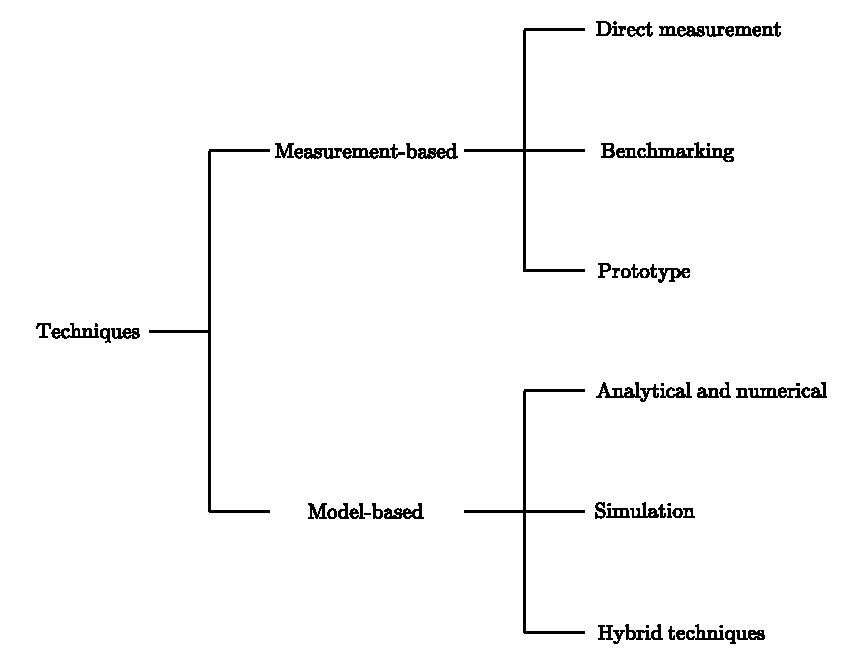
\includegraphics[width=\textwidth]{img/quality-evaluation.pdf}
	\caption{Quality Evaluation techniques.}
	\label{fig: Quality Evaluation techniques}
\end{figure}

\noindent
The most common and useful solution to evaluate system quality is \textbf{model-based approach}. The systems are complex, so it is useful to create an \textbf{abstraction of the systems called models}. The model-based are divided into three groups:
\begin{itemize}
	\item \definition{Analytical and numerical techniques} are based on the \textbf{application of mathematical techniques}, which usually exploit results coming from the theory of probability and stochastic process.
	\begin{flushleft}
		\textcolor{Green3}{\faIcon{check-circle} \textbf{Advantages}}
	\end{flushleft}
	\begin{itemize}
		\item Most \textbf{efficient}.
		\item \textbf{Accurate}.
	\end{itemize}
	\begin{flushleft}
		\textcolor{Red2}{\faIcon{thumbs-down} \textbf{Disadvantages}}
	\end{flushleft}
	\begin{itemize}
		\item \textbf{Available} only in very \textbf{limited cases}.
	\end{itemize}
	
	\item \definition{Simulation techniques} are based on the \textbf{reproduction of traces of the model}.
	\begin{flushleft}
		\textcolor{Green3}{\faIcon{check-circle} \textbf{Advantages}}
	\end{flushleft}
	\begin{itemize}
		\item Most \textbf{general}.
	\end{itemize}
	\begin{flushleft}
		\textcolor{Red2}{\faIcon{thumbs-down} \textbf{Disadvantages}}
	\end{flushleft}
	\begin{itemize}
		\item May be \textbf{less accurate}, especially when considering cases where rare events may occur.
		\item \textbf{Solution time} can also be \textbf{very long} if high accuracy is desired.
	\end{itemize}
	
	\item \definition{Hybrid techniques} \textbf{combine analytical/numerical methods with simulation}.
\end{itemize}

\newpage

\subsubsection{Queueing Networks}

\paragraph{Definition}

\definition{Queueing Network Modeling} is a particular approach to computer system modeling in which the \textbf{computer system is represented as a network of queues}. A \emph{network of queues} is a collection of \textbf{service centers}, which represent system \textbf{resources}, and \textbf{customers}, which represent \textbf{users} or \textbf{transactions}.\cite{lazowska1984quantitative}

\highspace
Some \example{examples} of queues in computer systems are:
\begin{itemize}
	\item CPU uses a time-sharing scheduler.
	
	\item A disk serves a queue of requests waiting to read or write blocks.
	
	\item A router on a network serves a queue of packets waiting to be routed.
	
	\item Databases have lock queues where transactions wait to acquire the lock on a record.
\end{itemize}

\begin{figure}[!htp]
	\centering
	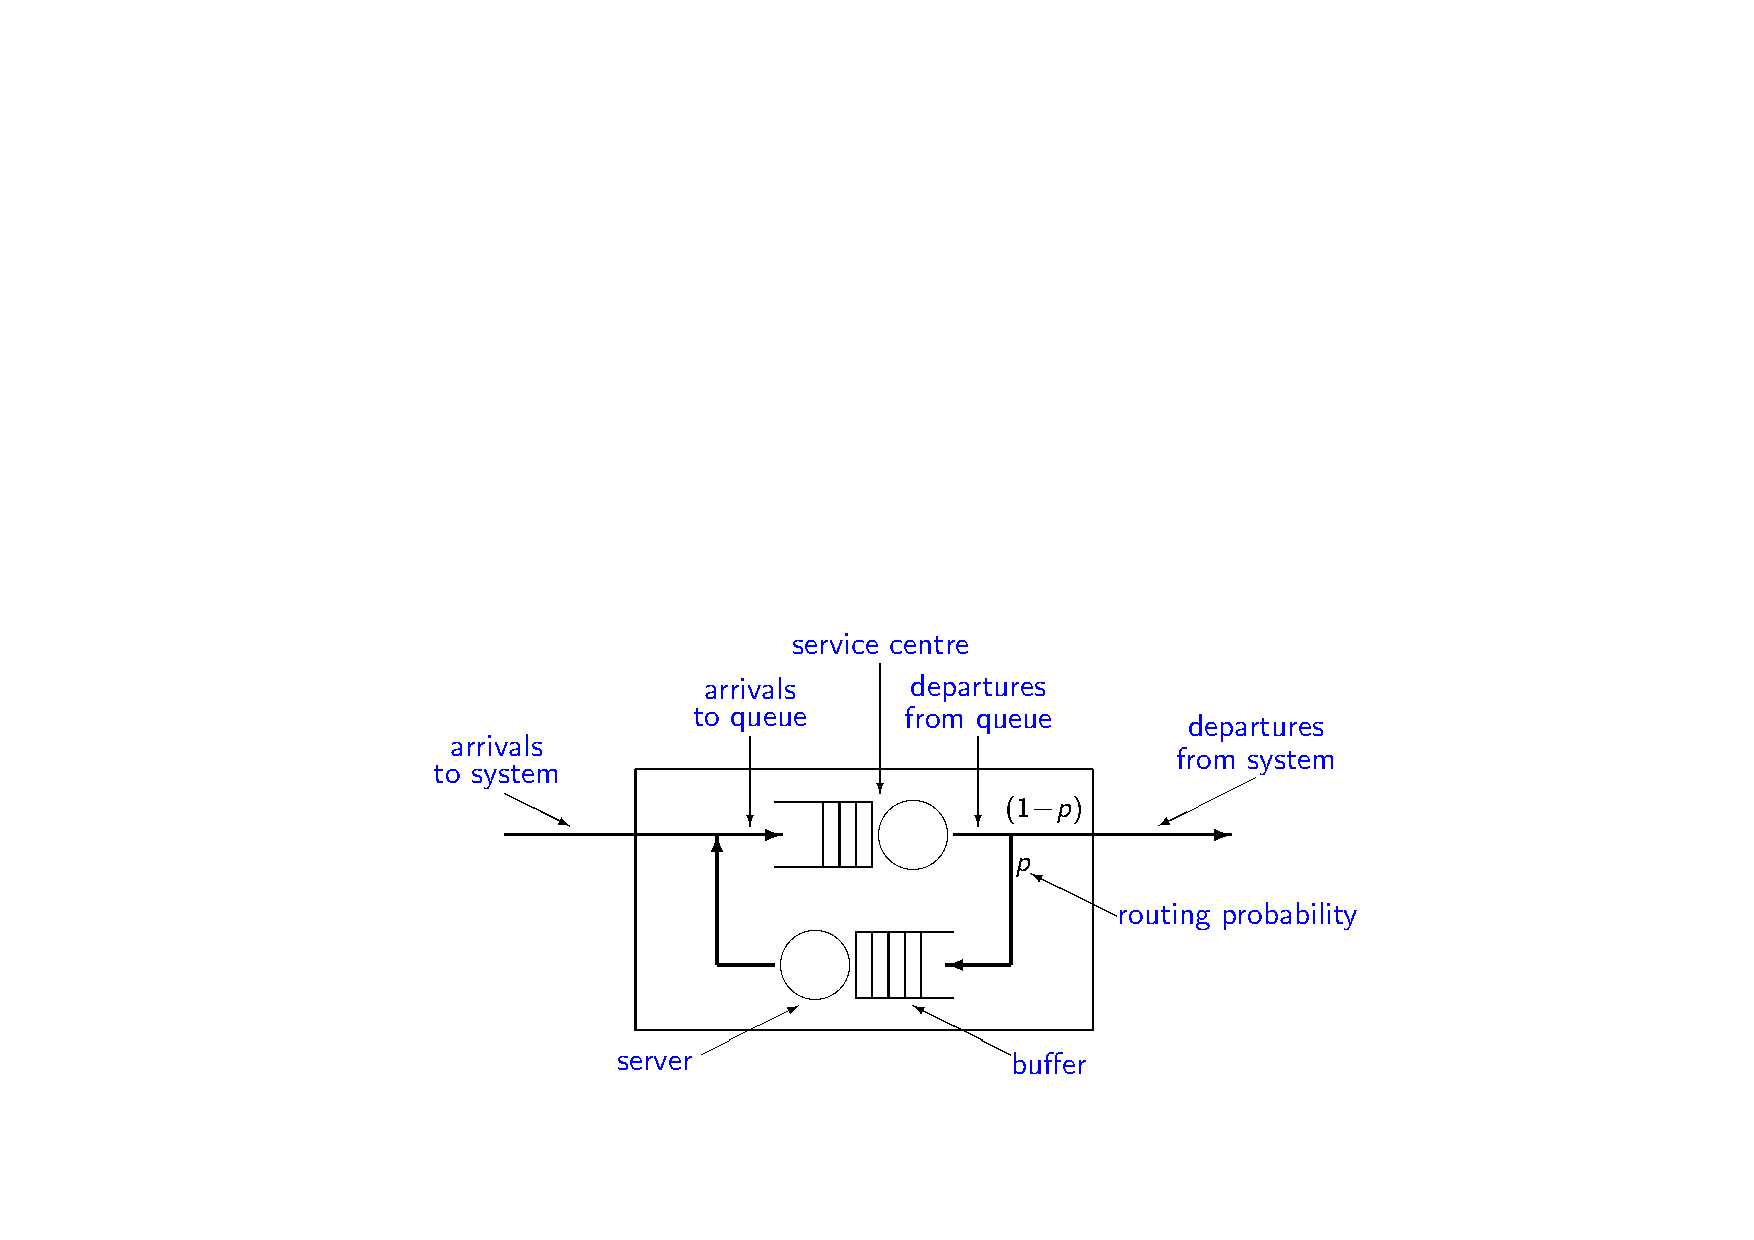
\includegraphics[width=\textwidth]{img/queueing-network-1.pdf}
	\caption{Queueing Network graphical representation.}
\end{figure}

\newpage

\paragraph{Characteristics}

Queueing models are characterized by several aspects:
\begin{itemize}
	\item \textbf{\underline{Arrival}}. Arrivals \textbf{represent orders coming into the system}. They specify \emph{how fast}, \emph{how often}, and \emph{what types of jobs} the \textbf{station will service}. \textbf{Arrivals can come from}:
	\begin{enumerate}
		\item An external source.
		\begin{figure}[!htp]
			\centering
			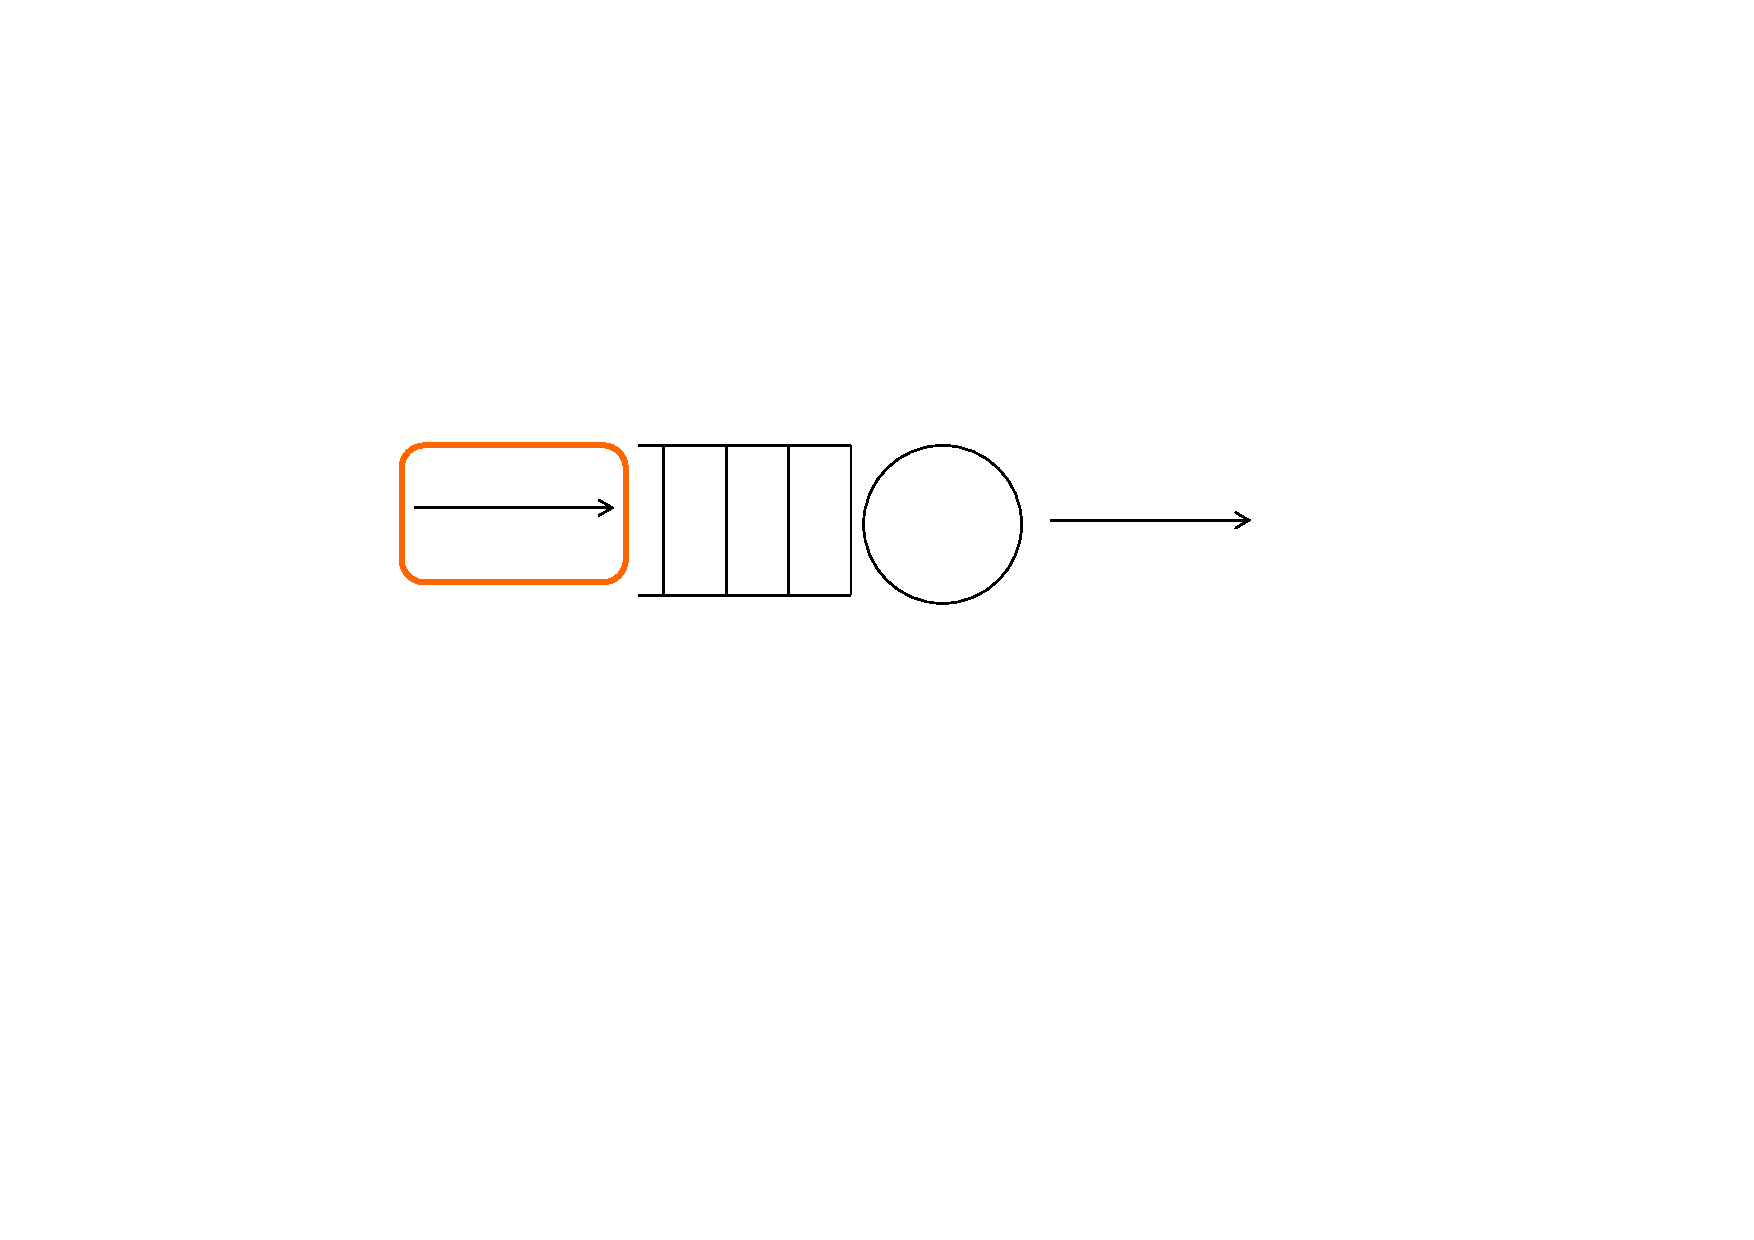
\includegraphics[width=.6\textwidth]{img/queueing-network-2.pdf}
		\end{figure}
		
		\item Another queue.
		\begin{figure}[!htp]
			\centering
			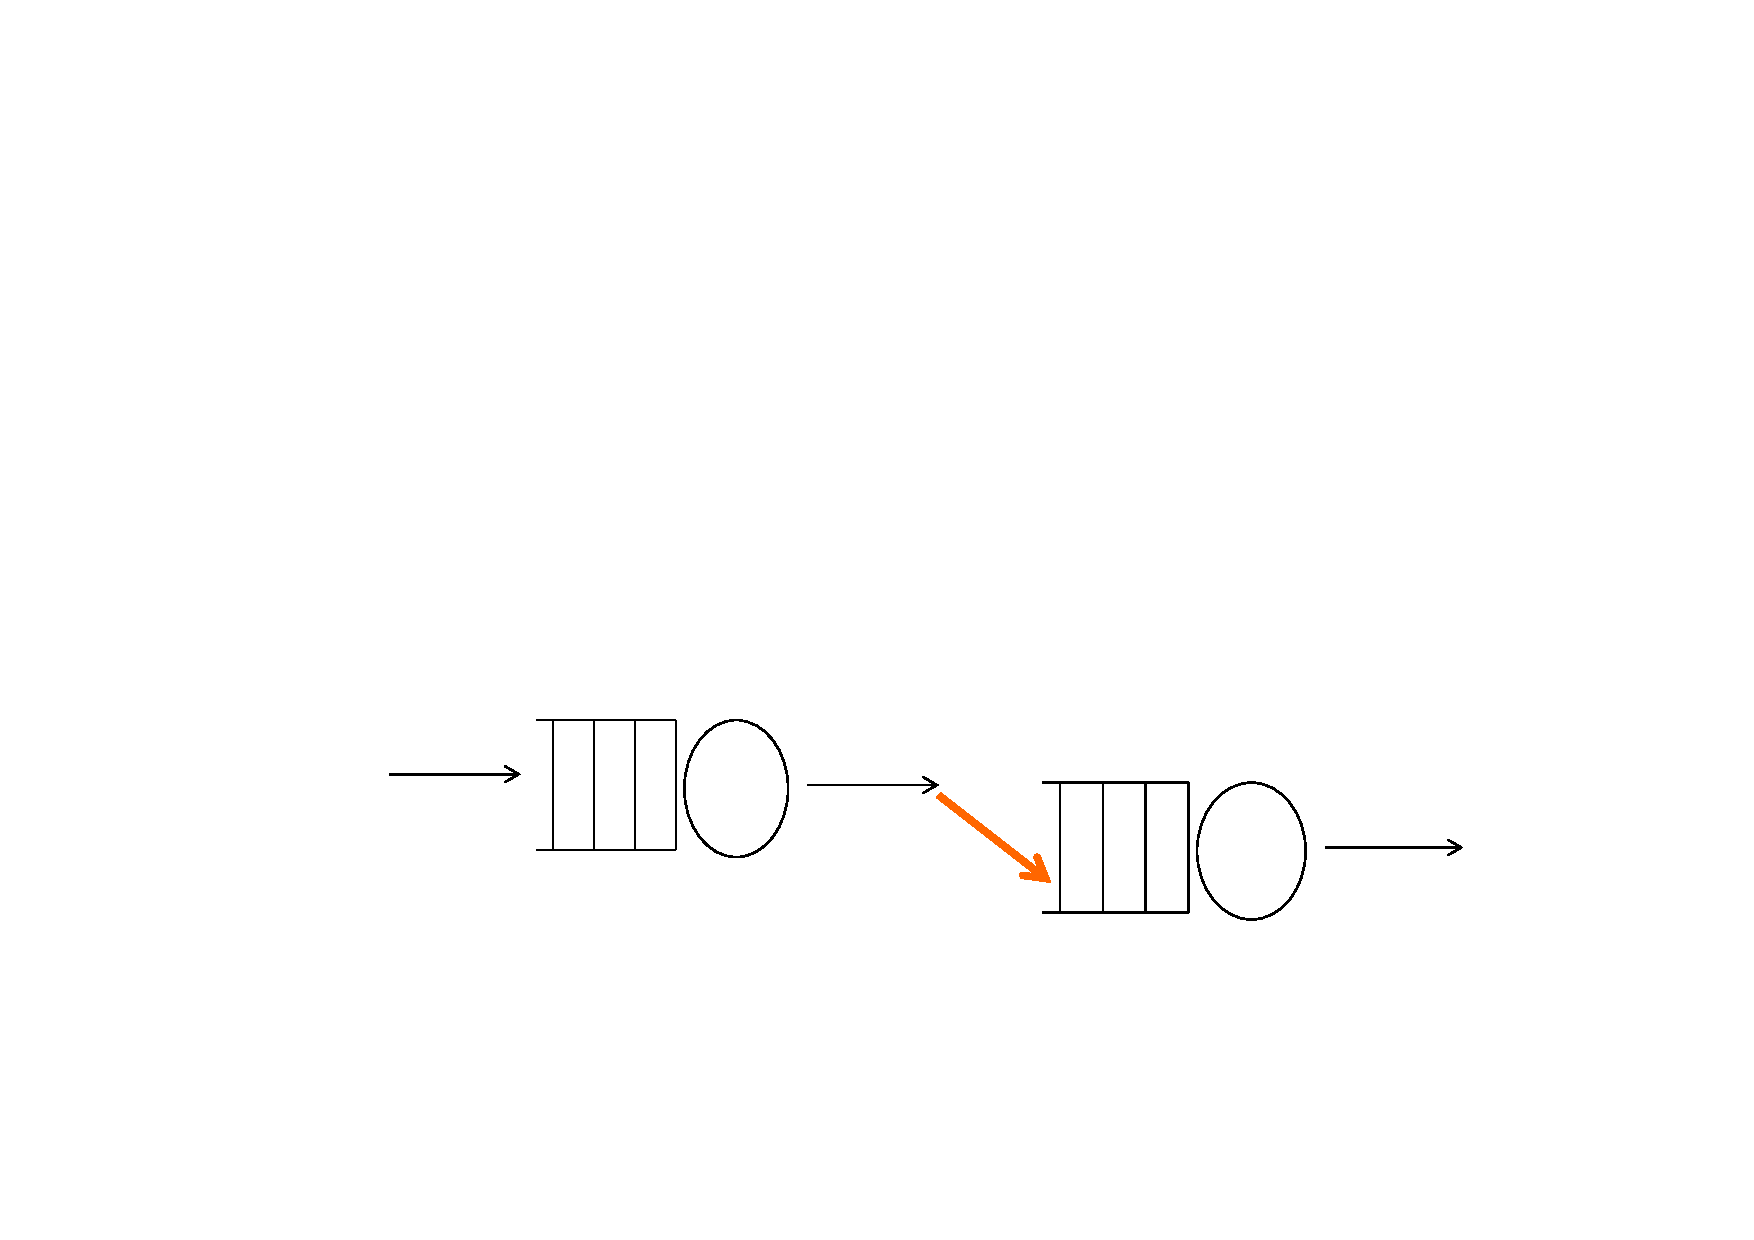
\includegraphics[width=.8\textwidth]{img/queueing-network-3.pdf}
		\end{figure}
		
		\item The same queue, through a loopback arc.
		\begin{figure}[!htp]
			\centering
			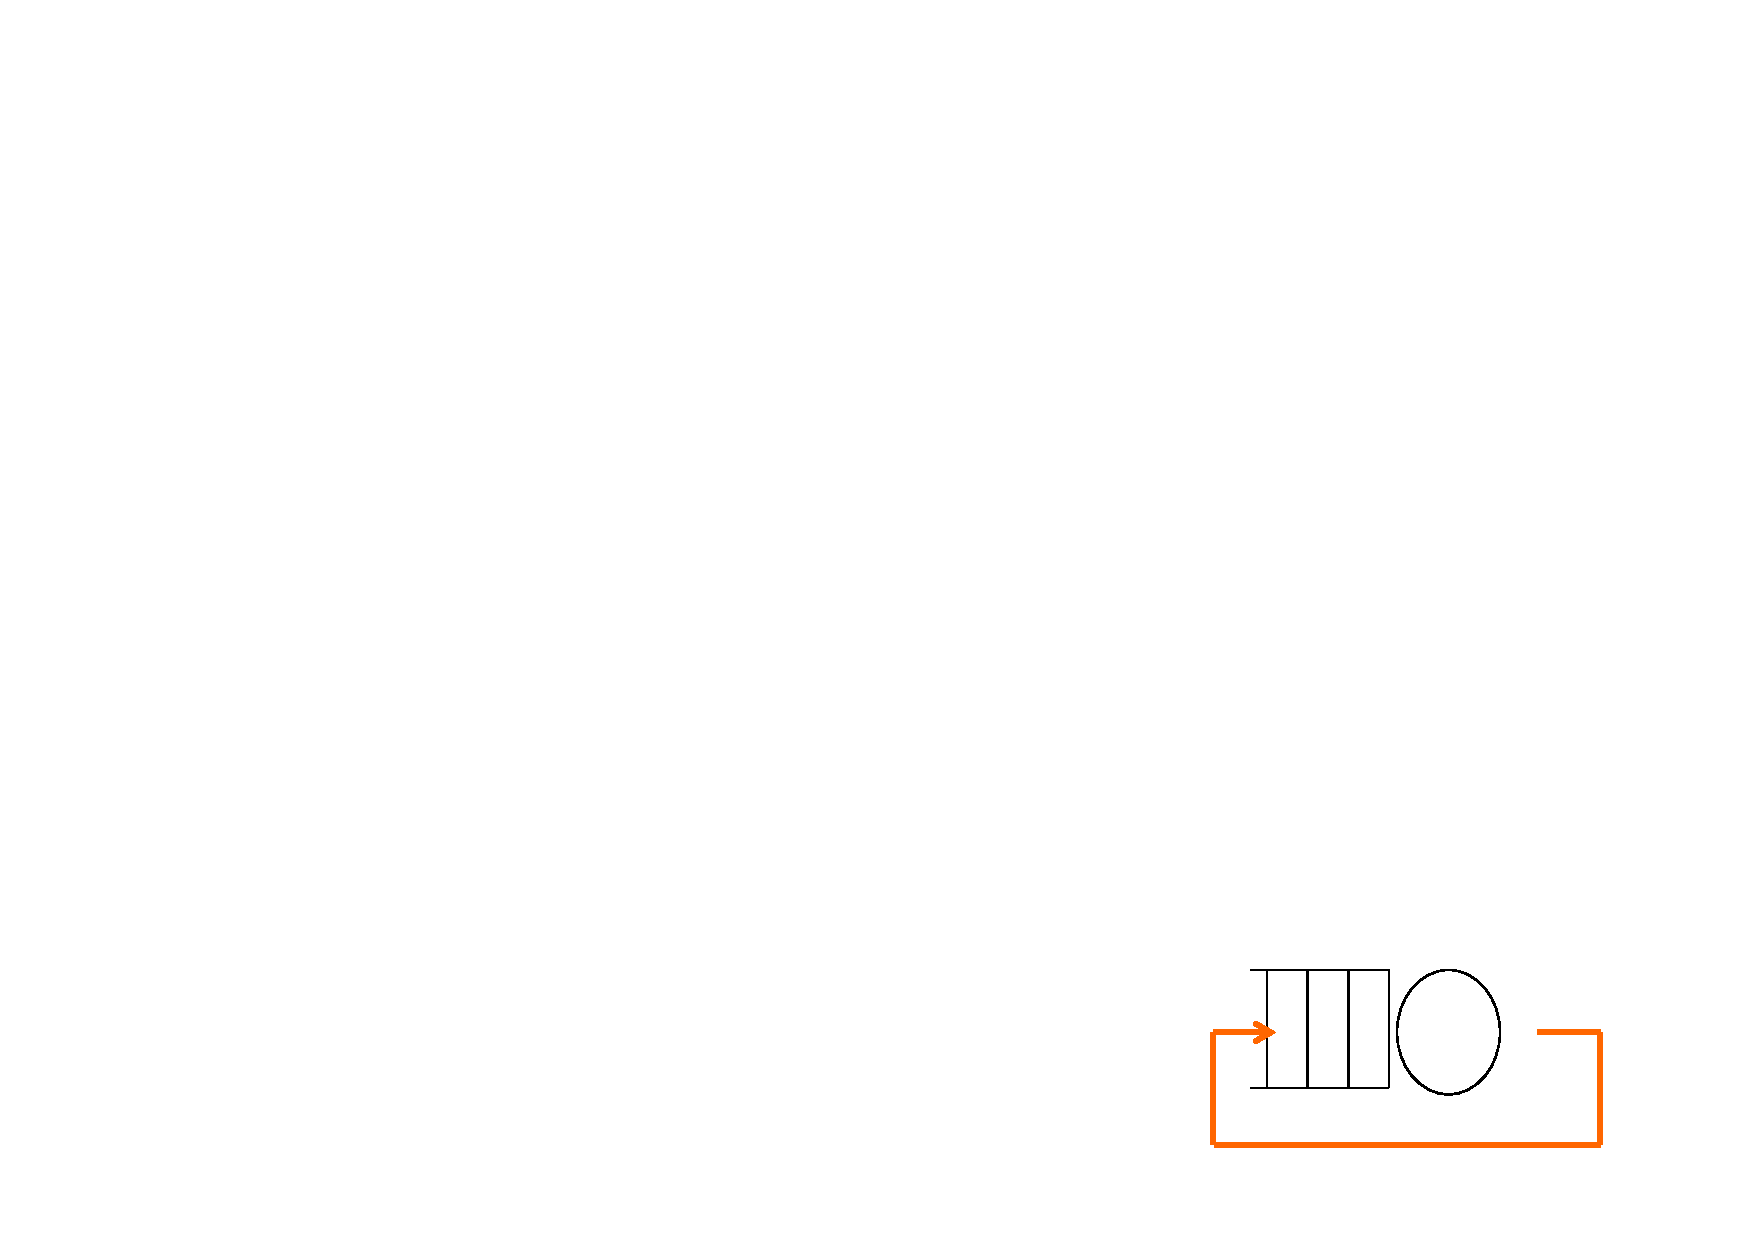
\includegraphics[width=.3\textwidth]{img/queueing-network-4.pdf}
		\end{figure}
	\end{enumerate}
	
	\item \textbf{\underline{Service}}. Service \textbf{represents the time a job spends being served}. The server does the job, but the number of servers can be different:
	\begin{itemize}
		\item \textbf{Single server}. It has the ability to serve \textbf{one client at a time}. \textbf{Waiting customers remain in the buffer} until they are selected for service. Finally, the \textbf{next customer is selected depending on the service discipline}.
		\begin{figure}[!htp]
			\centering
			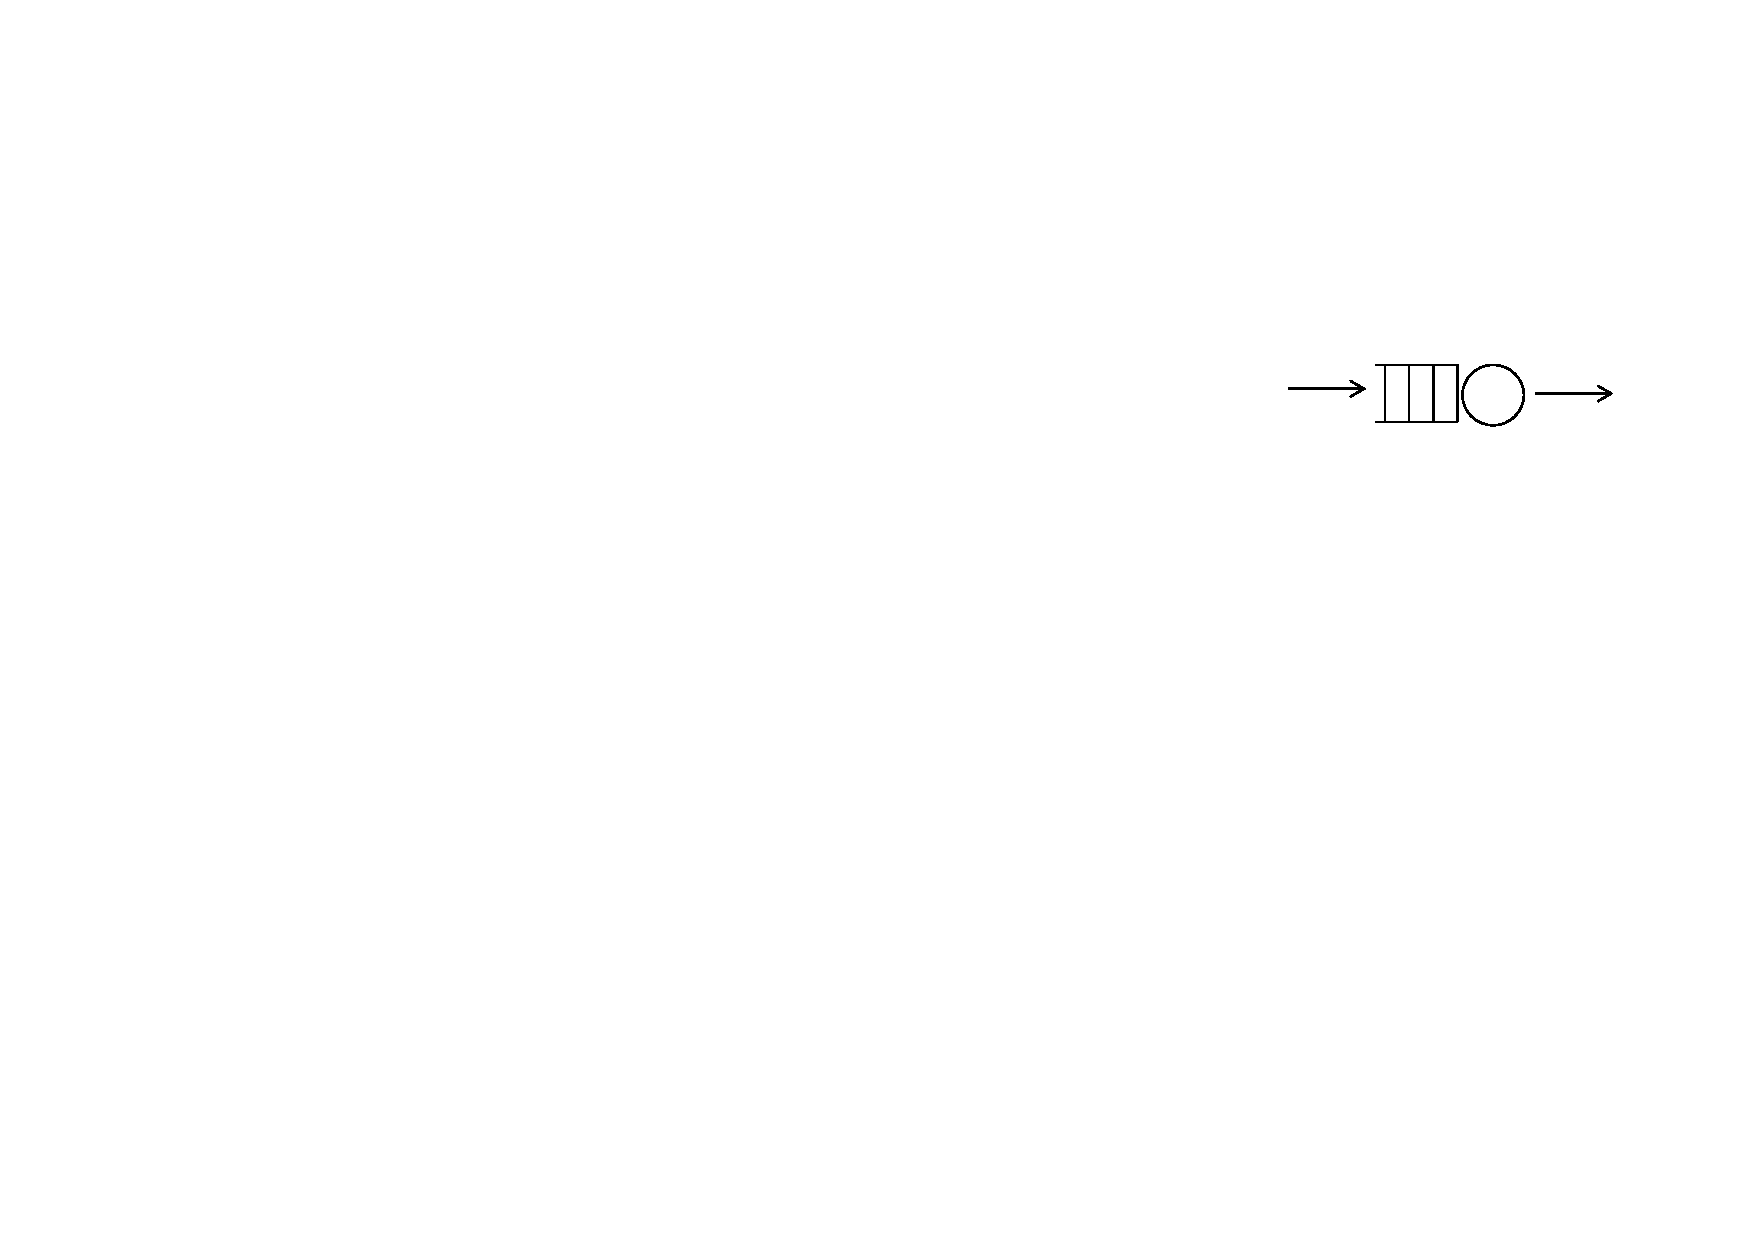
\includegraphics[width=.3\textwidth]{img/queueing-network-5.pdf}
		\end{figure}
		
		\item \textbf{Infinite servers}. There are always at least \textbf{as many servers as there are customers}, and each \textbf{customer can have a dedicated server}. As a consequence, there is \underline{no queuing} (and \underline{no buffer}).
		\begin{figure}[!htp]
			\centering
			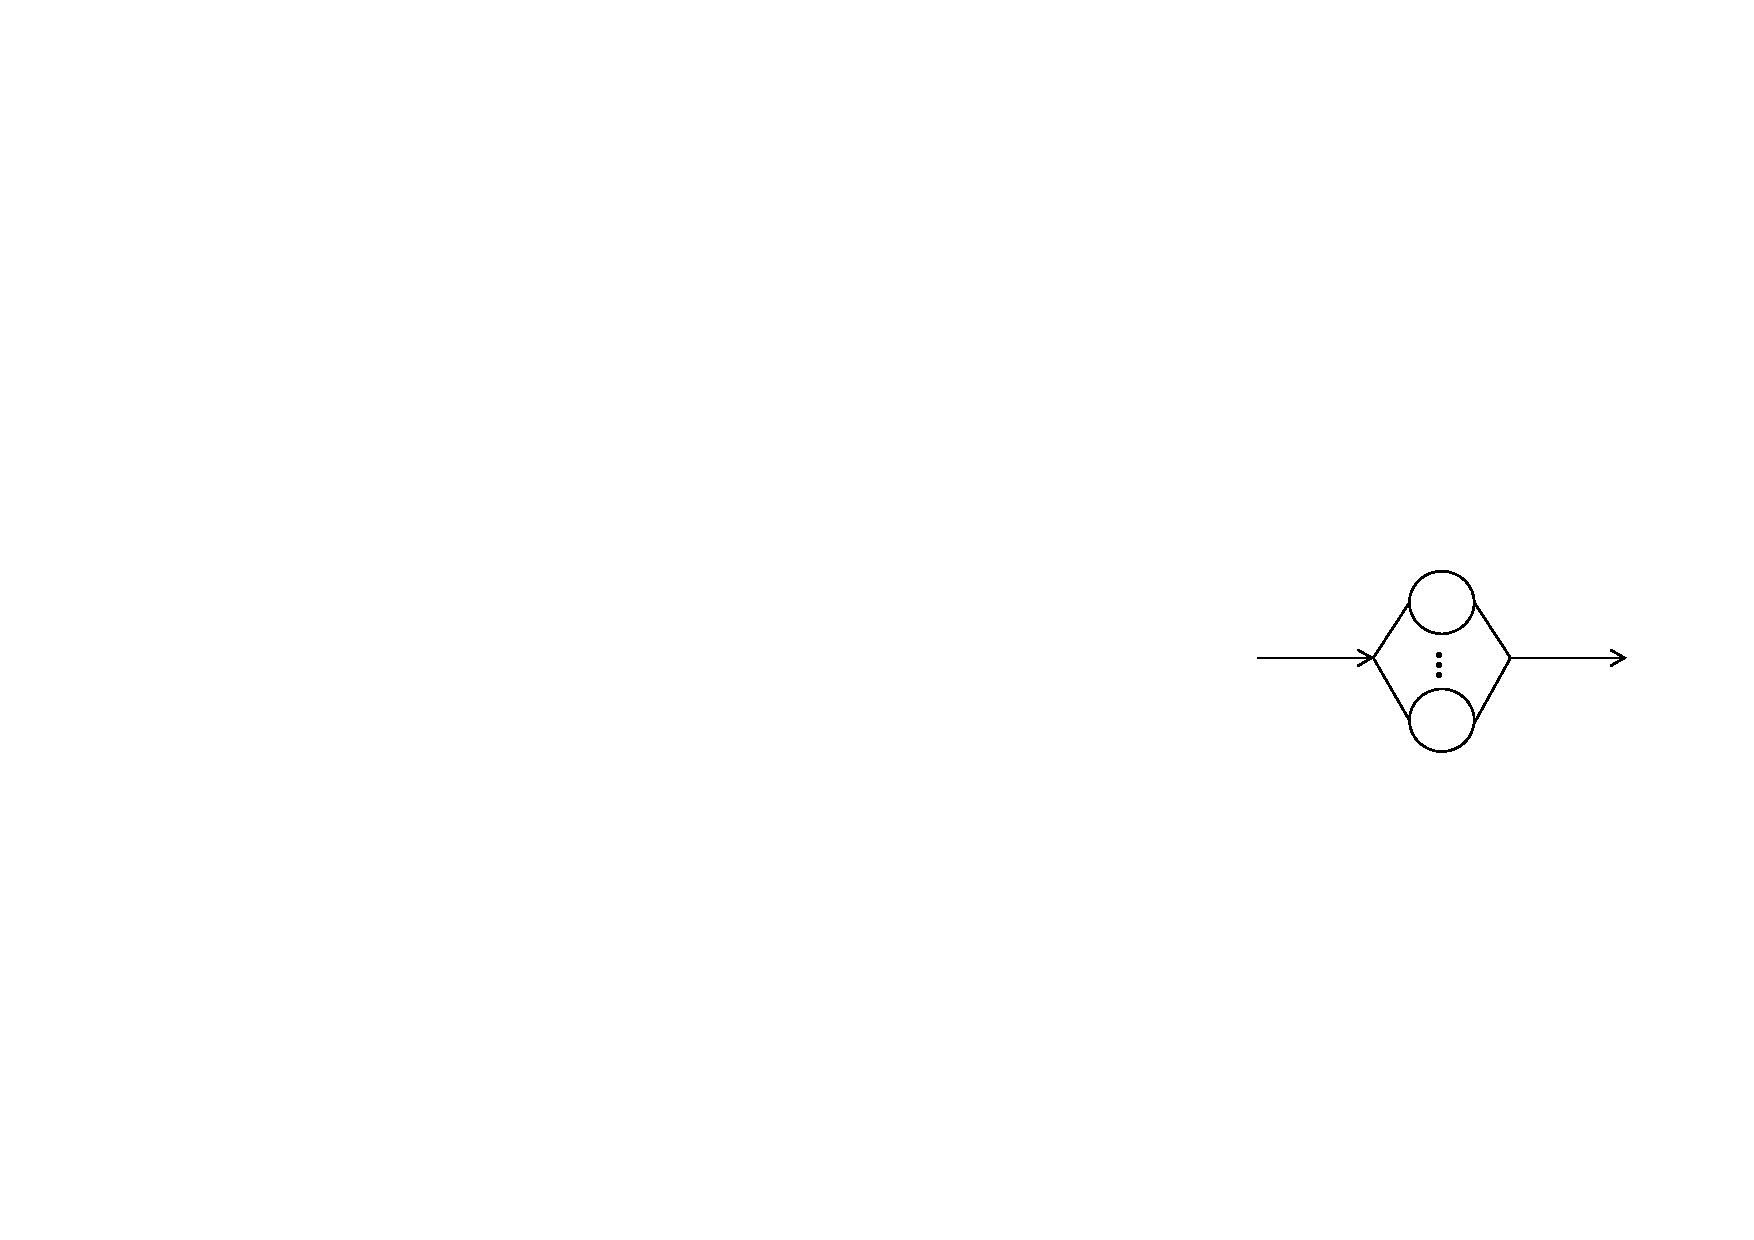
\includegraphics[width=.3\textwidth]{img/queueing-network-6.pdf}
		\end{figure}
		
		\item \textbf{Multiple servers}. There is a \textbf{fixed number of servers} (c in the figure below), each of which can \textbf{serve one customer at a time}. 
		\begin{itemize}
			\item \texttt{Number of customers in the system} $\le$ \texttt{number of servers} $\Rightarrow$ \textbf{no queuing}.
			\item \texttt{Number of customers in the system} $>$ \texttt{number of servers} $\Rightarrow$ the additional \textbf{customers must wait in the buffer}.
		\end{itemize}
		\begin{figure}[!htp]
			\centering
			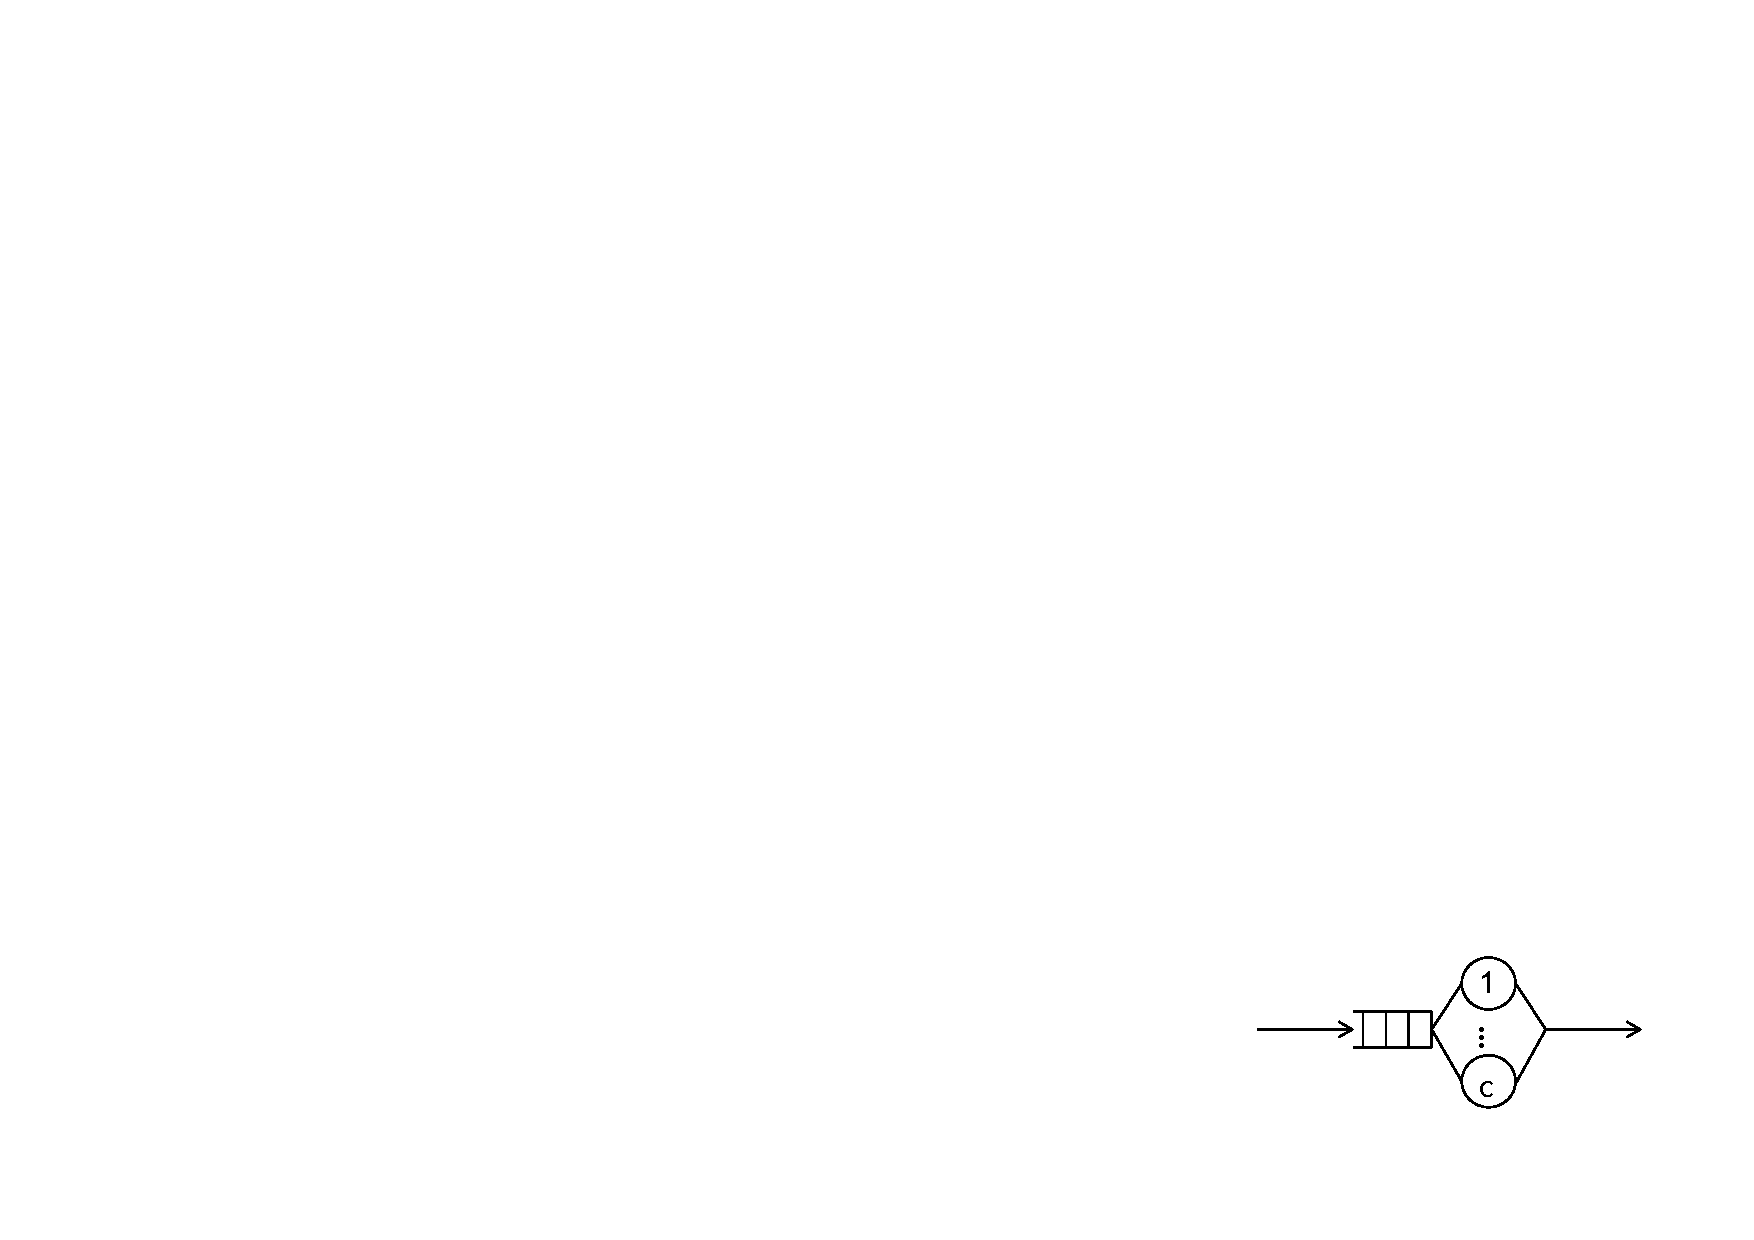
\includegraphics[width=.3\textwidth]{img/queueing-network-7.pdf}
		\end{figure}
	\end{itemize}
	
	\item \textbf{\underline{Queue}}. If \textbf{jobs exceed the parallel processing capacity of the system}, they are \textbf{forced to wait in a buffer}.
	
	When the job currently in service leaves the system, one of the jobs in the queue can now enter the free service center.
	\definition{Service Discipline}/\definition{Queuing Policy} \textbf{determines which of the jobs in the queue will be selected to start its service}.
	
	\item \textbf{\underline{Population}}. Ideally, members of the population are indistinguishable from one another. When this is not the case, we divide the population into \textbf{classes whose members all exhibit the same behavior}. Different classes differ in one or more characteristics, e.g. arrival rate, service demand. Identifying different classes is a task of workload characterization.
	
	\item \textbf{\underline{Routing}}. For many systems, we can view the system as a collection of resources and devices, with customers or jobs circulating between them.
	
	We can associate a service center with each resource in the system and then route customers between the service centers.
	
	After being serviced at one service center, a customer can move on to other service centers, following a pre-defined pattern of behavior according to the customer's needs.
	
	A queueing network can then be represented as a graph where the nodes represent the service centers k and the arcs represent the possible transitions of users from one service center to another. Nodes and arcs together define the network topology.
	
	Whenever \textbf{a job has several possible alternative routes after completing service at a station}, an appropriate selection policy must be defined.
	
	The policy is also called the \definition{Routing Algorithm}. The most important routing algorithms are:
	\begin{itemize}
		\item \definition{Probabilistic Routing Algorithm}. \textbf{Each path is assigned a probability of being chosen by the job that left the station in question}.
		
		\item \definition{Round Robin Routing Algorithm}. The \textbf{destination chosen by the job rotates among all possible existing destinations}.
		
		\item \definition{Join the shortest queue Routing Algorithm}. \textbf{Jobs can query the queue length of the possible destinations and choose the one with the least number of jobs waiting to be served}.
	\end{itemize}
\end{itemize}
With important definition of routing, we can say that a \textbf{network} can be:
\begin{itemize}
	\item \textbf{\underline{Open}}. Customers can come from or go to any external environment.
	\item \textbf{\underline{Closed}}. A fixed population of customers remains within the system.
	\item \textbf{\underline{Mixed}}. There are classes of customers within the system that exhibit both open and closed patterns of behavior.
\end{itemize}
An additional graphical notation is:
\begin{figure}[!htp]
	\centering
	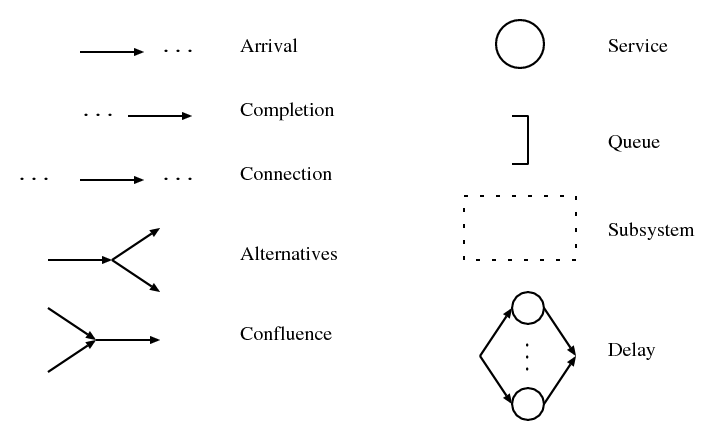
\includegraphics[width=\textwidth]{img/queueing-network-8.png}
\end{figure}

\begin{examplebox}[: Open Networks]
	A client server system, dealing with external arrivals (classical three tier architecture).
	
	Provide a QN model of the system and evaluate the overall throughput considering that the network delay is negligible with respect to the other devices and two different cases:
	\begin{enumerate}
		\item The only thing we know is that each server should be visited by the application.
		\item In the second case we know that the application \textbf{after visiting the web server} requires some operations at \textbf{the application server} and then \textbf{can go back} to \textbf{the web server} and \textbf{leave} the system \textbf{or} can require service at the \textbf{DMBS} and then \textbf{go back} to the \textbf{application server}.
	\end{enumerate}
	\begin{center}
		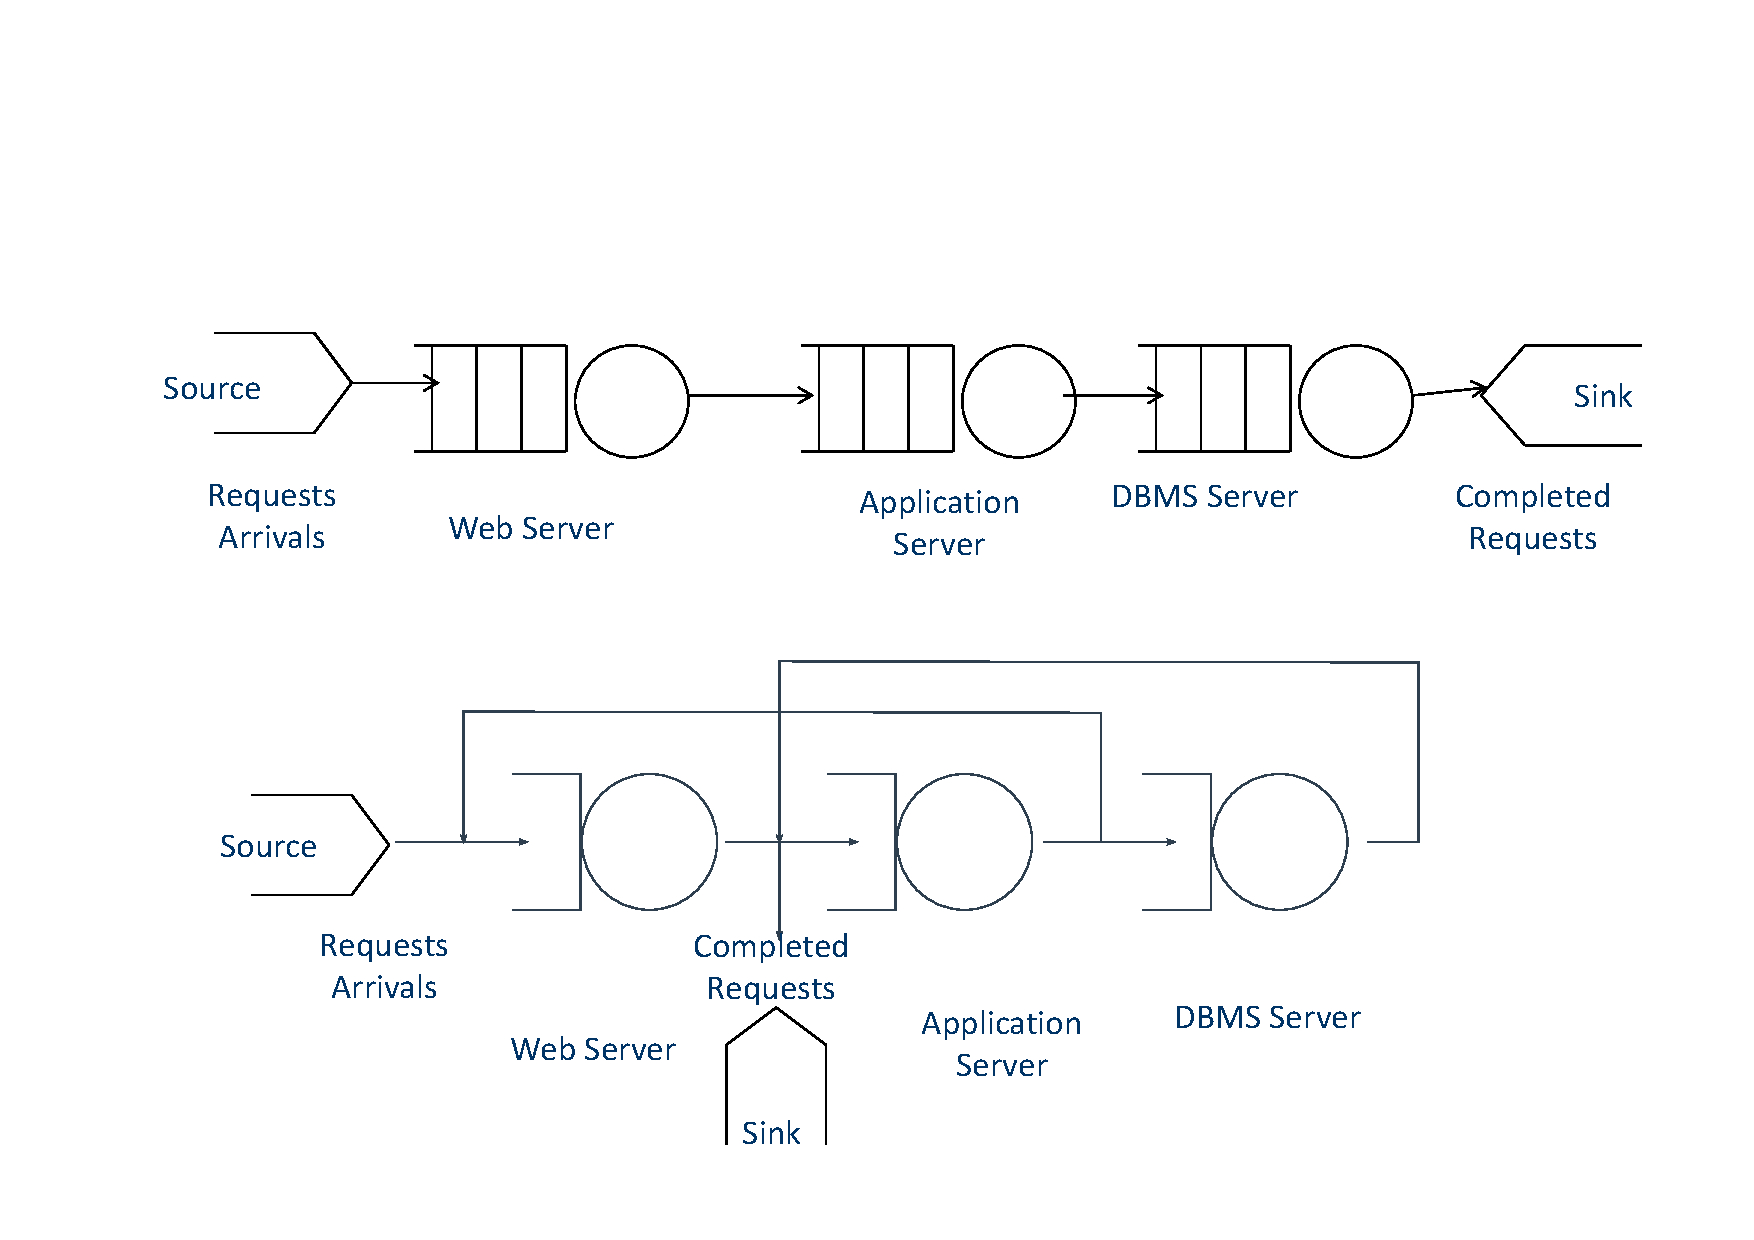
\includegraphics[width=\textwidth]{img/queueing-network-9.pdf}
	\end{center}
\end{examplebox}

\begin{examplebox}[: Closed Networks]
	A client server system, \textbf{with a finite number of customers} (classical three tier architecture and not accessible from outside).
	
	Provide a QN model of the system and evaluate the system throughput considering that Network delay is negligible with respect to the other devices. Model the two different cases previously described.
	\begin{itemize}
		\item First scenario
		\begin{center}
			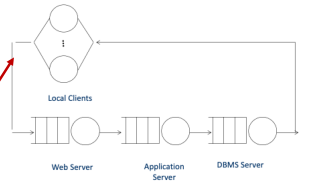
\includegraphics[width=.65\textwidth]{img/queueing-network-10.png}
		\end{center}
		
		\item Second scenario
		\begin{center}
			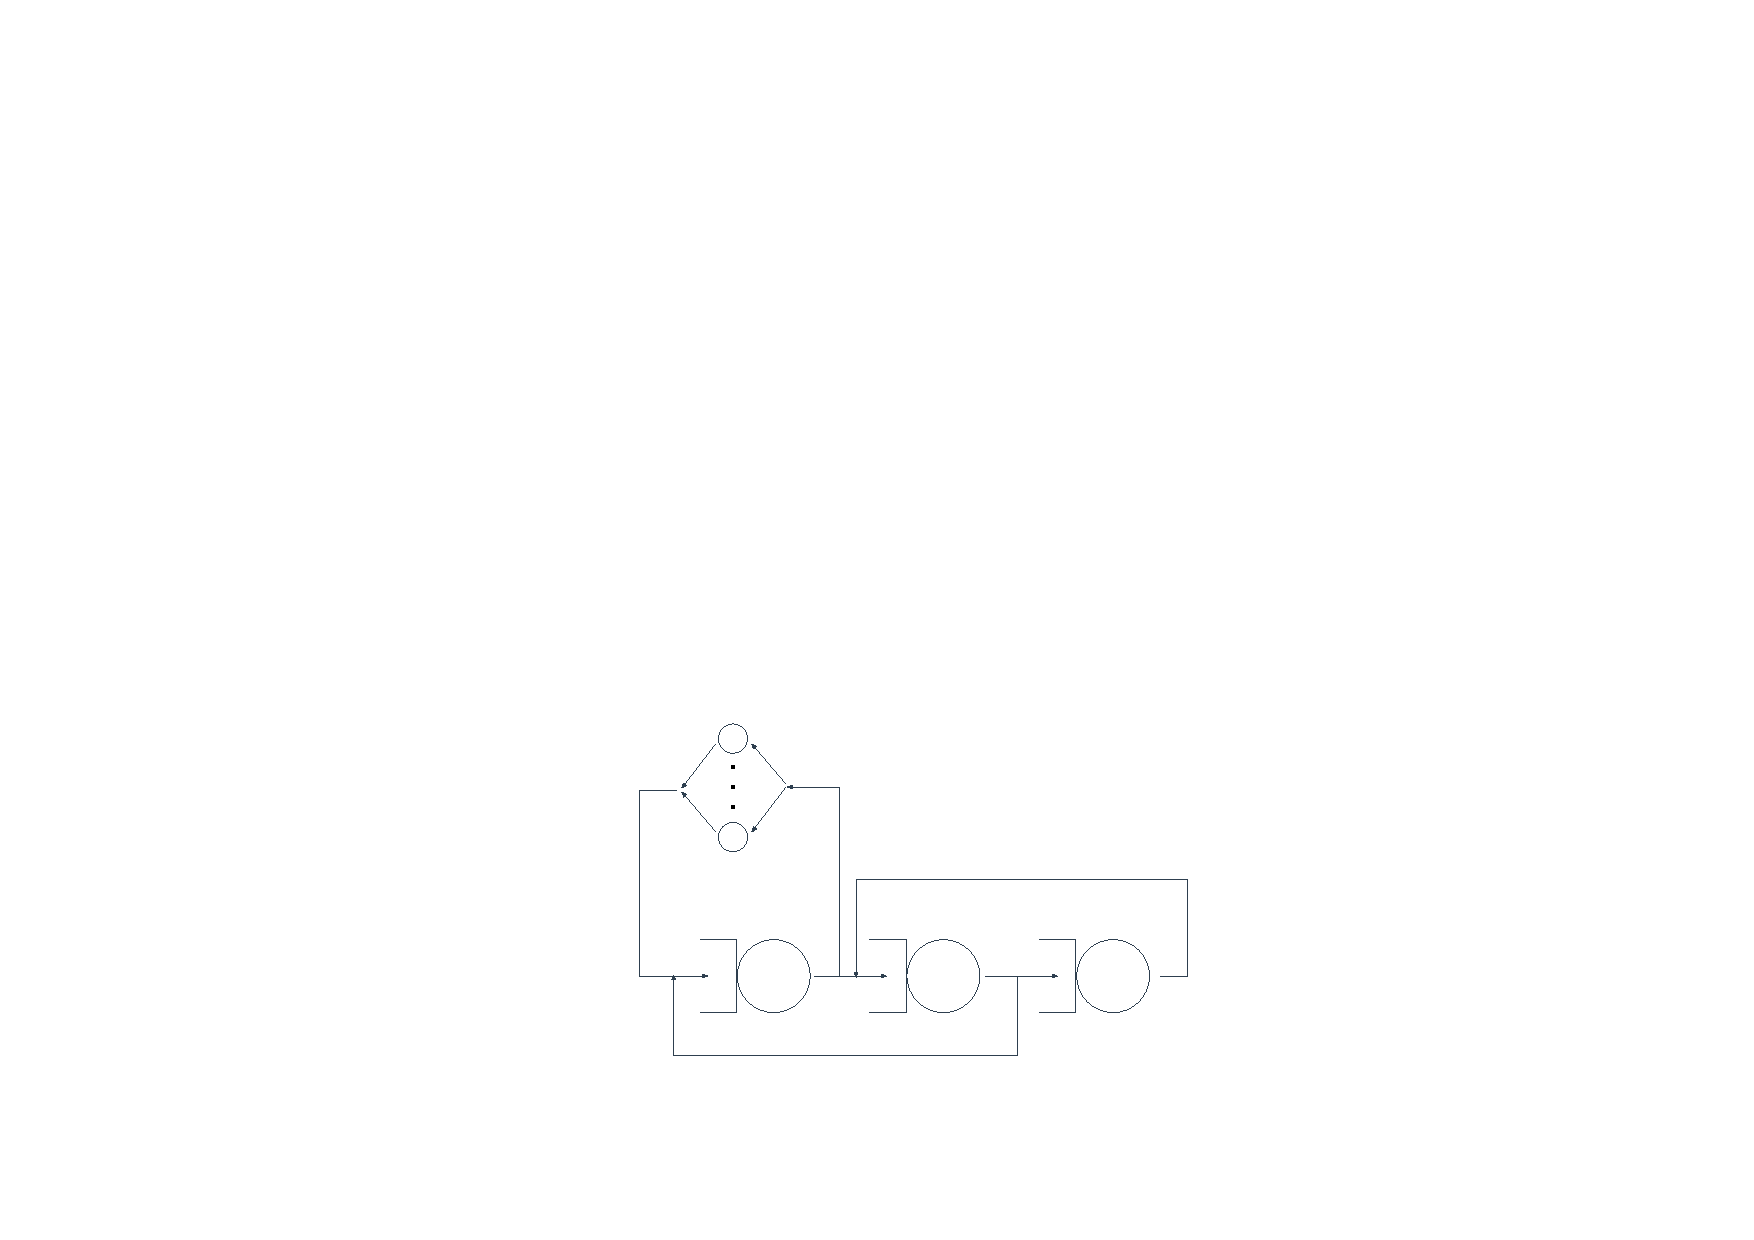
\includegraphics[width=.6\textwidth]{img/queueing-network-11.pdf}
		\end{center}
	\end{itemize}
\end{examplebox}